% I'm not totally sure, if this should be described together or seperate, but somehow or SCRUM approach and the Redmine
% stuff should be mentioned somewhere before the developing part and as this are probably only three pages or somethin
% it probably could be integrated here
\chapter{Features}\label{chap:features}

\section{Notifications and Comments}

The following section describes an important part for registered users, the notification system and the opportunity for adding comments basically on any resource in the system.

\subsection{Recent activity stream}
It displays the most recent events in the portal in the order they happened. Each activity (figure \ref{fig:activity-stream-single-activity}), one line in the stream, consists of 3 parts: meta information about the activity itself, information about the initiator and comments. The content of each of these parts is being determined automatically, when a new notification is being persisted to the database.

Besides the initiator information and comments, each activity has an own title, description and icon. These meta information texts can be edited in the portal in the 'Administration' > 'Acions' section. Although it is not possible to remove them, because the action references are being used hard-coded within the system. That means a set of notifications is provided and can be ouput anywhere in the workflow.

\begin{figure}[!h]
  \centering
  \fbox{
    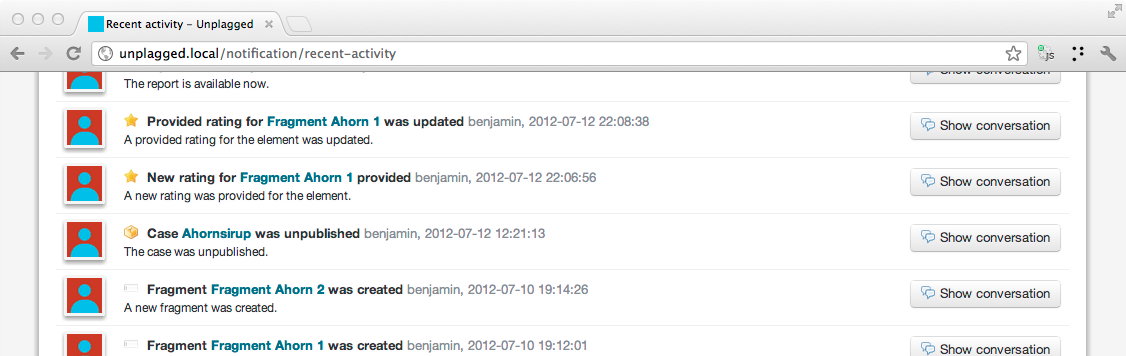
\includegraphics[width=0.97\textwidth]{images/feature-activity-stream.png}
  }
  \caption{Single activity in the activity stream}
  \label{fig:activity-stream-single-activity}
\end{figure}

The following code snippet shows, how to create a new notification when a new automatic plagiarism detection report was created. The static method takes in 3 parameters: a unique name for the notification type, the content object related to the notification and a user object, as the third parameter. A list of all available notification types can either be found in the previousely mentioned actions section or in the scripts/build/initdb.php file, where all notifcation types are being declared.

\begin{lstlisting}[caption=Creating a notification for a created report]
Unplagged_Helper::notify("detection_report_created", $report, $report->getUser());
\end{lstlisting}

Unplagged does have an extensive role and permission management. Therefore the grant on each resource is being verified, before it is being displayed in the activity stream. Usually the resource related to the notification is the resource where the permission check is being performed on. Although in some cases, e.g. when rating a fragment, the resource will be the rating itself, but the permission check is done on the fragment. In this case the notify-method is being called with a fourth, optional parameter, another resource, in this case the fragment. When the user has access on the fragment, all ratings can be accessed as well, automatically.

\subsection{Comments plugin}

Comments are simply a small text related to a specific user and a resource. They can be used to share ideas on an object collaboratively. The most prominent part at Unplagged, where comments are being used, is the activity stream. A comment can be added by any user having access to the notification. 

\begin{figure}[!h]
  \centering
  \fbox{
    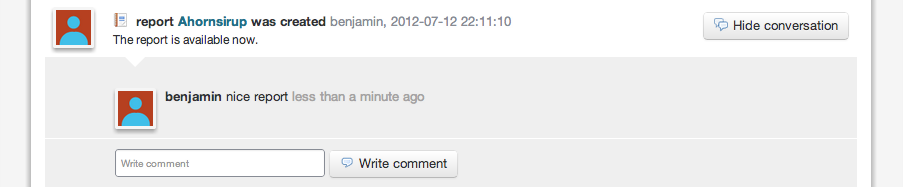
\includegraphics[width=0.97\textwidth]{images/feature-comment.png}
  }
  \caption{Creating a comment on a resource}
  \label{fig:creating-a-comment}
\end{figure}

For providing a better workflow to the user, the comments can be refreshed and added in place. That means, the position where the user scrolled to in the browser does not get affected. The in-place refreshing is being realized through AJAX. The comments container is being loaded empty and displaying a small loading image only. Not before the user clicks the 'show conversation' button, the comments are being fetched through a post request to the server. Whenever the result is being fetched completely, the spinner graphic is being hidden and the comments are being appended. The parsing of the comments markup is being done in Javascript as well. So the server requests are kept small and the server can return JSON only without any HTML.

\begin{lstlisting}[caption=Refreshing the comments of a resource]
	target.show();
      conversation.hide();
      loading.slideDown(800, function() {
        // get the whole conversation
        $.post('/notification/conversation', {
          'source': sourceId
        }, function(data) {
          if(!data.errorcode) {
            conversation.html("");
            $.each(data, function(index, value) {
              conversation.append(renderConversation(value));
            });
            loading.slideUp(800, function() {
              conversation.slideDown(300);
            });
          } else {
            conversation.html('<div class="comment">' + data.message + '</div>');
            loading.slideUp(800, function() {
              conversation.slideDown(300);
            });
          }
        }, "json");
\end{lstlisting}

\begin{lstlisting}[caption=Creating the markup of a single comment]
function renderConversation(data, target) {
    var tpl;
    
    switch(data.type) {
      case 'comment':
        tpl = '<div class="comment">' +
        '<div class="image"><img class="avatar-small" src="' + data.author.avatar + '" /></div>' +
        '<div class="details">' +
        '<div class="title"><b>' + data.author.username + '</b> ' + data.text + 
        ' <span class="date">' + data.created.humanTiming + '</span>' +
        '</div>' +
        '</div>' +
        '</div>';
        break;
    }
    if(!target) {
      return tpl;
    } else {
      target.append(tpl);
    }
  }
\end{lstlisting}

\section{Fragments}
@benjamin

\subsection{Creating a fragment}
@benjamin

the-old-way

two-column view

\subsection{Rating a fragment}
@benjamin

\section{Barcode}
@benjamin

\section{User avatar}
@elsa

\subsection{Avatar cropping}
@benjamin

\section{Automatic Plagiarism Detection Webservice}
@benjamin
\subsection{PlagAware}
@benjamin

\section{Permission and role management}
@dominik
types of permission, types of roles

\subsection{Collaborators}
@benjamin

new role created from global case role